\documentclass{pnu-survey}

%%%%%%%%%%%%%%%%%%%%%%%%%%%%%%%%%%%%%%%%%%%%%%%
% 필요한 패키지가 있다면 하단에 적어주세요.
%%%%%%%%%%%%%%%%%%%%%%%%%%%%%%%%%%%%%%%%%%%%%%%
% 이미지 및 그래프 관련 패키지
\usepackage{graphicx}
\usepackage{float}
\usepackage{subfloat}
\usepackage{subfigure}
\usepackage{lscape}
\usepackage{enumitem}

% \usepackage[compact]{titlesec}

% 수학 기호 관련
\usepackage{gensymb}
\usepackage{amsmath}
\usepackage{amssymb}
\usepackage{amsthm}
\usepackage{exscale}
\usepackage{textcomp}

\newcommand{\cl}[1]{\textcircled{\scriptsize #1}}

% 알고리즘 표현
\usepackage{algorithmic}
\usepackage{algorithm}

% customize algorithmic environment
\renewcommand{\algorithmicrequire}{\makebox[40px]{\hfill\textbf{Input :}}}
\renewcommand{\algorithmicensure}{\makebox[40px]{\hfill\textbf{Output :}}}

% 테이블 관련
\usepackage{array}
\usepackage{tabulary}
\usepackage{multirow}
\usepackage[table]{xcolor}
\usepackage{ctable}
\usepackage{booktabs}
							
% 제목, 저자, 요약
\title{4세대 K-Pop 아이돌 뮤직비디오의 특징}
\author{한상곤(sangkon@pusan.ac.kr)}
\abstract{
K-Pop에 대한 관심이 높아지고, YouTube 등과 같은 동영상 플랫폼을 기반으로 한 영상 미디어에 대한 접근 방식에 많은 변화가 일어났다. 짧은 시청 시간을 가지고 있는 영상 플랫폼의 특성을 고려해서 음악의 핵심 부분을 1분 정도 편집한 영상을 별도로 작성한다. 4세대 아이돌의 특징을 규정하는 세계관을 표현하기 위해서 다채로운 색채 뿐만 아니라 자막과 같은 특수효과를 적극적으로 도입하고 있다. 영상 플랫폼에 따른 미디어 전략이 4세대 아이돌의 뮤직비디오에 영향을 주었고, 동시에 이런 영향은 4세대 아이돌의 특징을 규정하는 뚜렷한 특징으로 자리잡았다. 본 논문은 4세대 아이돌과 이전 세대의 아이돌의 뮤직비디오의 특징을 비교함으로써 기존 미디어 전략을 이해하고, 향후 미디어 전략에 대한 논의를 계속하고자 한다.
}

\begin{document}

\maketitle

\section{서론}

Aliquam maximus fermentum tellus, a condimentum purus commodo ac. Duis metus tellus, venenatis sit amet mi et, hendrerit blandit justo. Aenean elementum odio eu sapien mollis pulvinar. In posuere metus aliquet, mattis mi vitae, porttitor enim. Vivamus ullamcorper vulputate condimentum. Morbi quam purus, feugiat eget ultricies vitae, ultrices vitae ligula. Nunc non risus eget purus ultricies aliquet. Duis magna tortor, viverra non semper dignissim, imperdiet quis urna. Maecenas quam nisi, vehicula in massa ac, rutrum ornare nulla. Proin luctus erat ut metus ornare, id ultrices erat ullamcorper. Sed consectetur leo id felis ornare finibus. Duis eget condimentum magna. Phasellus a urna lobortis, mattis dolor id, facilisis elit. Vestibulum vel accumsan felis.

\section{본론}

Morbi a imperdiet enim~\cite{syh}. Donec cursus, sem et consectetur ornare, lectus felis pellentesque nunc, a consectetur quam est et nisi. Curabitur tristique mattis ante a vulputate. Mauris a justo et diam commodo finibus in nec mi. Ut consectetur, sem eget fringilla congue, quam ligula fermentum tellus, et accumsan mi lacus quis purus. Pellentesque rutrum pretium arcu finibus congue. Fusce ex ante, auctor eu convallis a, lobortis vel eros. Phasellus dapibus eu nunc vitae porttitor. Nam quis fermentum quam. Aliquam tempus nulla id arcu vehicula consectetur. Morbi dictum diam quam, quis hendrerit purus luctus eu. Mauris in accumsan dolor, vel mattis turpis. Etiam commodo massa arcu, eget finibus sem feugiat in.

표 \ref{tab:datasets}과 같이 표를 작성할 수 있다.
\begin{table}[!ht]
\centering
\setlength{\belowcaptionskip}{5pt}
\caption{실험 데이터의 주요 통계적 수치}
\label{tab:datasets}
\begin{tabular}{@{}lrrrr@{}} 
\toprule
{\bfseries Dataset} & $|\mathcal{D}|$ & ${\rm avg}(|x|)$ & $|\mathcal{U}|$ & ${\rm avg}(|I_i|)$ \\
\midrule
LAST.FM			&134,949	&  4.8	& 47,295	& 13.8\\
LAST.FM 4G		&			& 11.2	& 44,272	& 34.3\\
DBLP			&1,298,016	&  8.6	&381,450	& 29.3\\
TREC			&348,566	& 77.1	&298,302	& 90.1\\
UKBENCH			&10,200		&425.7	&533,412	&  6.9\\
\bottomrule
\end{tabular}
\end{table}

\textbf{Nam fringilla enim ante, laoreet interdum sapien convallis a.} Vestibulum sit amet risus a nisi tincidunt auctor a quis tortor. Maecenas ante lacus, venenatis non quam eget, vulputate egestas libero. Nam non diam justo. Mauris et risus hendrerit nibh bibendum egestas. Pellentesque purus arcu, tristique quis ornare ac, vehicula scelerisque leo. Nullam ultrices ante odio, et suscipit felis dictum vitae. Nam urna urna, dapibus at mi et, imperdiet varius ante.

그림 \ref{fig:example1}과 같이 그림을 삽입할 수 있다. 아래 구조를 잘 확인해서 그림을 작성하세요. 될 수 있으면 snippet 형태로 사용하시길 권해드립니다.

\begin{figure}[!ht]
\centering
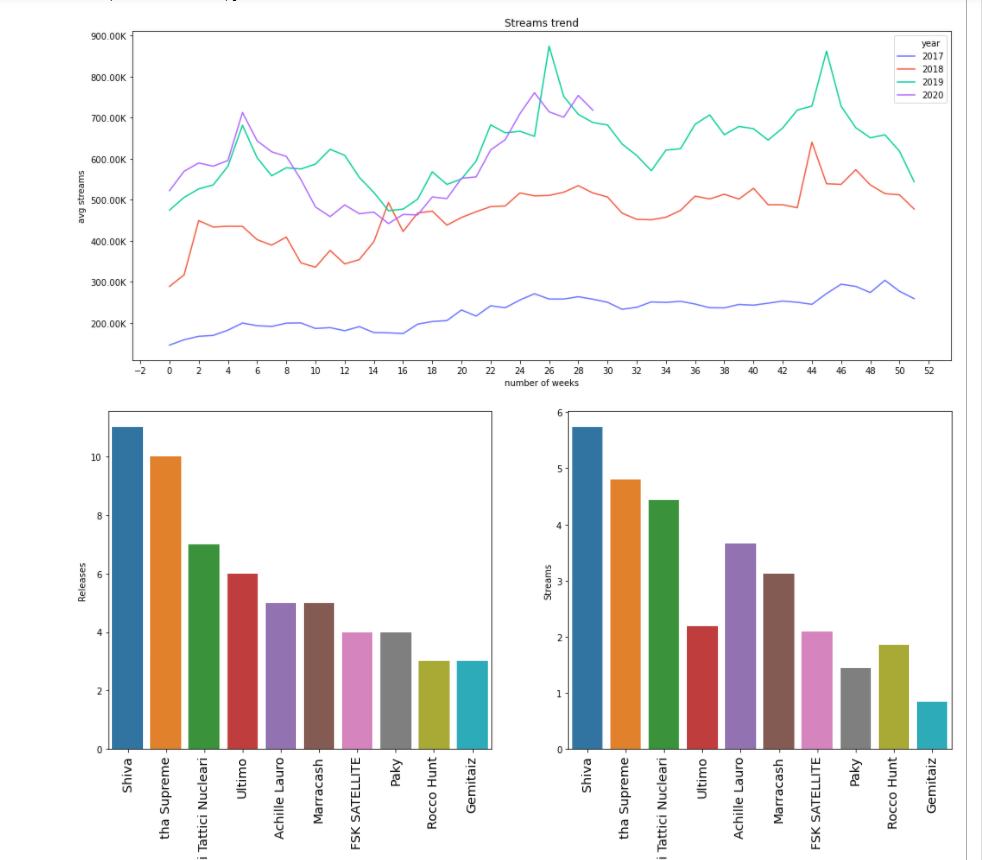
\includegraphics[width=0.4\textwidth]{img/fig1.png}
\caption{그림 예제}
\label{fig:example1}
\end{figure}
\index{figure}

알고리즘을 설명하는 것은 아래와 같은 형태로 진행하시면 됩니다. Algorithm \ref{alg:sum}과 같이 뭔가 있어보이는 형태로 작성이 가능합니다. 이 정도까지 오셨으면 출판도 고려해보면 좋겠네요.

\begin{algorithm}[!ht]
\label{alg:sum}
\caption[Short label]{\texttt{SumOnlyPositives}($\mathcal{D}$)}
\begin{algorithmic}[1]
\REQUIRE a set of real number $\mathcal{D}$ 
\ENSURE sum of all non-negative elements in $\mathcal{D}$ 
\STATE $O \leftarrow 0$
\FOR{\textbf{each} $x\in \mathcal{D}$ }
	\IF{$x > 0$}  
		\STATE $O \leftarrow O + x$
	\ENDIF
\ENDFOR
\RETURN $O$
\end{algorithmic}
\end{algorithm}

아, 수학 수식도 가능합니다. 아마, 수업시간에 별도로 다룰 예정입니다. 너무 걱정하지 마세요. 수식 
 \eqref{eq:eq1}과 같이 수식을 바로 참조할 수 있다.

\begin{equation}
\label{eq:eq1}
SumOnlyPositives(\mathcal{D}) = \sum_{\forall x \in \mathcal{D} \land x > 0 }x
\end{equation}

아, 항목이 필요하시면 아래와 구조를 참고하세요.

\begin{itemize}[itemsep=0pt,parsep=0pt]
  \item There are many variations of passages of Lorem Ipsum available, but the majority have suffered alteration in some form, 
  \item by injected humour, or randomised words which don't look even slightly believable. If you are going to use a passage of Lorem Ipsum, you need to be sure there isn't anything embarrassing hidden in the middle of text. All the Lorem Ipsum generators on the Internet tend to repeat predefined chunks as necessary, making this the first true generator on the Internet. It uses a dictionary of over 200 Latin words, combined with a handful of model sentence structures, to generate Lorem Ipsum which looks reasonable. The generated Lorem Ipsum is therefore always free from repetition, injected humour, or non-characteristic words etc.
\end{itemize}

\section{결론}

Quisque vestibulum, sapien at tristique rutrum~\cite{lsh}, massa quam blandit lectus, eu fermentum nibh quam et dui. Vivamus mattis nulla sit amet lectus venenatis tincidunt. Fusce sapien velit, facilisis a tempor vel, viverra at lacus. Sed quam diam, aliquet vel eros et, pellentesque vehicula sem. Etiam volutpat congue nisl. Vestibulum fringilla sem neque, vitae viverra tellus cursus et. Praesent vulputate tristique lectus, eu sollicitudin enim mattis nec.

\bibliographystyle{ieeetr}
\bibliography{ref}
\end{document}
